\documentclass[prb,aps,twocolumn,showpacs,10pt]{revtex4-2}
\usepackage{graphicx}
\usepackage{tikz}
\usetikzlibrary{arrows, shapes, positioning}
\usetikzlibrary{decorations.markings}
\usepackage{amsmath}
\usepackage{physics}


\begin{document}

\title {The nuclear many-body problem through the lenses of exactly solvable models}
\author{Jane Kim}
\date{\today}
\begin{abstract}

Background, Purpose, Methods, Results, and Conclusions. 
\end{abstract}
\maketitle


\section{INTRODUCTION}

A common goal in science is to understand how properties of systems emerge from the fundamental interactions between their constituents and their environment. Regardless of the system in question, we aim to construct simple models to aid our understanding before adding layers of complexity to more accurately depict reality. This systematic approach allows us to build conceptual frameworks with varying degrees of detail. Although the models themselves are often designed to be as simple as possible for the sake of interpretability, the resulting conclusions are rarely as straightforward. Thus, exactly solvable models serve as an important tool to not only understand the systems we study, but the methods we use to study them.


Nearly all scientific endeavors involve objects consisting of baryonic matter, the vast majority of which comes neatly packaged in atomic nuclei. Therefore, unraveling the mystery of nuclei is a necessary step in understanding the observable universe. In this review, we will investigate the nuclear many-body problem using two exactly solvable models: the Lipkin model and the seniority model. In particular, we will compare how several commonly used many-body methods perform, helping to predict the behavior of these methods when applied to more complicated models which lack analytical solutions. 


The implementations of all the methods in this 
*** github repo ***

\section{THE NUCLEAR MANY-BODY PROBLEM}

*** maybe don't call this Abody? ***
The general form of an $A$-body nuclear hamiltonian is given by
\begin{equation}
\hat{H} = \sum_{i=1}^A -\frac{\hbar^2}{2m_i} \nabla_i^2 + \sum_{i<j}^A v(i,j),
\end{equation}
where $i$ represents the degrees of freedom of the $i$th nucleon, such as position, spin, and isotopic spin, and $v(i,j)$ represents a two-body interaction. Ideally, we would like to solve the many-body Schr\"odinger equation
\begin{equation}
\hat{H} \Psi(1,...,A) = E \Psi(1,...,A),
\end{equation}
for the full microscopic picture, but this is a lofty goal for all but the smallest of nuclei. 

There are several things to notice here. First, we assume that the nucleus is a quantum mechanical system. Although this is obvious, this means we need to consider how the uncertainty and Pauli exclusion principles combine with the nuclear forces to give rise to the observed structure and density of nuclei. We also assume that the nucleons are the appropriate degrees of freedom at this scale, rather than the quarks and gluons they are composed of. Next, we have only included two-body interactions, but it is possible that up to A-body interactions are involved. Finally, relativistic effects are neglected since the velocities of the nucleons are somewhat small ($(v/c)^2 \sim 1/10$). [R\&S]

All things considered, even the "full" nuclear hamiltonian in equation (1) is a simplified version of the actual problem. Yet it is still difficult to solve (2) for an arbitrary two-body interaction due to the immense computational cost which grows exponentially with the size of the system. To bypass these restrictions, we resort to approximate methods. But that leaves us to wonder: how do we know if these methods provide reasonable results? This is why exactly solvable models are useful. Even if the model itself does not realistically portray a nucleus, they can be used to test the computational methods that would be applied to a more realistic model.

The models in Sections III and IV build upon the shell model of the nucleus. Similar to the electrons in an atom, the nucleons fall into the lowest-energy shells allowed by the Pauli exclusion principle. However, these shells emerge from the interactions between the nucleons themselves rather than an external central field. This shell structure is corroborated by the existence of the so-called "magic numbers", i.e. the number of protons or neutrons contained in a particularly stable nucleus. 

\section{LIPKIN MODEL}

Many of the interesting properties of different nuclei are largely determined by the nucleons sitting in the outermost shell. Let us imagine that the last $j$-shell of a nucleus has $N$ nucleons of the same type. The remaining nucleons are stuck in the interior, forming a stable core whose effects we will cautiously ignore. Let us further assume that the shell just above the Fermi surface has the same $j$-value as the shell just below. Then the model hamiltonian can be described by $N$ nucleons interacting in a two-level system with $\Omega=2j+1$ available spots in each level:
\begin{equation}
\hat{H}_{LM} = \frac{1}{2} \epsilon \sum_{m \sigma} \sigma a_{m\sigma}^+ a_{m\sigma} - \frac{1}{2} V \sum_{m m' \sigma} a_{m\sigma}^+ a_{m'\sigma}^+ a_{m'-\sigma} a_{m-\sigma}.
\end{equation}
The $\epsilon$ in the first term is the energy spacing between the two levels. The second term essentially counts how many ways pairs of particles can be moved directly up or down between the levels, then scales the contribution to the hamiltonian with an attractive interaction parameter $V$. Note that the above description of the model assumes $N \leq \Omega$, but the following solutions are valid for $N > \Omega$ as well. 
\begin{figure}
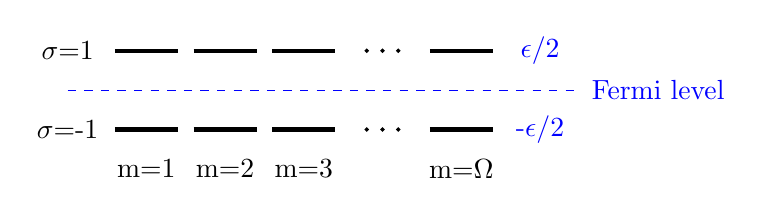
\begin{tikzpicture}

\foreach \x in {0, 1, 2, 4}
	\foreach \y in {0, 1}
		\draw[ultra thick] (\x+0.1,\y) -- (\x+0.9,\y);

\filldraw[black] (3.3, 0) circle [radius=0.02];
\filldraw[black] (3.5, 0) circle [radius=0.02];
\filldraw[black] (3.7, 0) circle [radius=0.02];
\filldraw[black] (3.3, 1) circle [radius=0.02];
\filldraw[black] (3.5, 1) circle [radius=0.02];
\filldraw[black] (3.7, 1) circle [radius=0.02];

\node at (-0.5, 0) {$\sigma$=-1};
\node at (-0.5, 1) {$\sigma$=1};
		
\node at (0.5, -0.5) {m=1};
\node at (1.5, -0.5) {m=2};
\node at (2.5, -0.5) {m=3};
\node at (4.5, -0.5) {m=$\Omega$};

\draw[dashed, blue] (-0.5, 0.5) -- (6, 0.5);
\node[blue] at (7, 0.5) {Fermi level};
\node[blue] at (5.5, 0) {-$\epsilon/2$};
\node[blue] at (5.5, 1) { $\epsilon/2$};

\end{tikzpicture}
\caption{Level scheme of the Lipkin model.}
\end{figure}

\subsection{Exact Methods}

\subsubsection{Configuration-Interaction}

To solve the full Lipkin model (LM) problem, we need to diagonalize the hamiltonian (3) in some basis. A naive approach could be to use the configuration-interaction (CI) basis and consider every possible way $N$ particles could be arranged in the 2$\Omega$ single-particle levels shown in FIG. 1. Since the $m$-degeneracy is ignored in this treatment, this basis can equivalently be applied to any system of $N$ particles arranged in any $2\Omega$ single-particle states, i.e. the dimension of the hamiltonian is always $2\Omega\choose N$. If we add up the dimensions for each possible $N$, we obtain the dimension of Fock space for the Lipkin model via the binomial theorem: $\sum_{N=0}^{2\Omega} {2\Omega\choose N} = 2^{2\Omega}$.

This approach is agnostic, meaning we did not impose any additional information that is specific to our chosen model. As a consequence, we must work in a much larger space, making even moderate-sized problems unreachable without extensive computational resources. For instance, we would need to consider ${2\Omega\choose N} = 184756$ configurations for $\Omega=N=10$, compared to the 36 states we would need in the quasi-spin basis. Once the entire hamiltonian is constructed, we would then need to diagonalize the full matrix, which is again a computationally heavy task. Many redundancies in the resulting spectra occur, i.e. there are extra zero eigenvalues. Therefore, a better basis would involve grouping the configurations based on the symmetries of the problem.

\subsubsection{Quasi-Spin}

As suggested above, let us imagine taking any configuration in the CI basis and flipping any two $m$-labels. If we obtain a different configuration, we place it in the same "group" as the first. Proceeding in this way, we split the vast collection of configurations into symmetry-dictated groups, significantly simplifying the problem. The configurations in any given group have the same characteristics, so we will henceforth view these groups as many-body states rather than the configurations within them. ** review this ** K+- moves between groups? 

Now that we have demonstrated the intuition behind mapping a brute force approach to a symmetry-guided approach, we will formalize this mapping by rewriting the Lipkin model hamiltonian in terms of quasi-spin operators:
\begin{equation}
\hat{H}_{LM} = \epsilon \hat{K}_0 - \frac{1}{2} V (\hat{K}_+ \hat{K}_+ + \hat{K}_- \hat{K}_-),
\end{equation}
where
\begin{align}
\hat{K}_0 &= \frac{1}{2} \sum_{m=1}^\Omega (a_{m+}^+ a_{m+} - a_{m-}^+ a_{m-} ),\\
\hat{K}_+ &= \sum_{m=1}^\Omega a_{m+}^+ a_{m-}, \\
\hat{K}_- &= (\hat{K}_+)^+.
\end{align}
These operators satisfy the commutation relations of angular momenta,
\begin{align}
&[\hat{K}_+, \hat{K}_-] = 2 K_0,\\
&[\hat{K}_0, \hat{K}_\pm ] = \pm \hat{K}_\pm,
\end{align}
and the total quasi-spin operator commutes with the hamiltonian,
\begin{align}
&\hat{K}^2 = \hat{K}_0^2 + \frac{1}{2} ( \hat{K}_+ \hat{K}_- + \hat{K}_- \hat{K}_+ ),\\
&[\hat{K}^2, \hat{H}_{LM}]=0,
\end{align}
making total quasi-spin $K$ a good quantum number. We can then write down the basis states $\ket{K, K_0}$ in a familiar way. The maximum value of $K$ is $K_{max} = N/2$ for $N\leq \Omega$ and $K_{max} = \Omega-N/2$ for $N > \Omega$. We obtain the remaining $K$ values by subtracting 1 from $K_{max}$ until $K_{min}=0$ or 1/2. For each value of $K$, there are $2K+1$ values of $K_0$ ranging from $-K$ to $K$ in integer steps. Applying the operators $\hat{K}_\pm$ on the basis states changes $K_0$ by $\pm 1$:
\begin{equation}
\hat{K}_\pm \ket{K,K_0} = \sqrt{K(K+1) - K_0(K_0\pm 1))} \ket{K,K_0 \pm 1}
\end{equation}
From this relation we can easily obtain explicit expressions for the non-zero matrix elements:
\begin{equation}
\bra{K,K_0'} \hat{H}_{LM} \ket{K,K_0} = \epsilon K_0 \delta_{K_0, K_0'}
\end{equation}
\begin{align*}
\bra{K,K_0'} &\hat{H}_{LM}\ket{K,K_0} \\
=& - \frac{1}{2}V \sqrt{K(K+1) - K_0(K_0\pm 1))} \\
&\sqrt{K(K+1) - (K_0 \pm 1)(K_0\pm 2))} \delta_{K_0\pm 2, K_0'}.\\
\end{align*}


Labeling the basis states by $K$ and $K_0$ implies that the hamiltonian matrix is block diagonal, with $K$ enumerating the blocks and $K_0$ enumerating the states within the blocks. By introducing the signature operator,
\begin{equation}
\hat{R} = e^{i \pi \hat{K}_0},
\end{equation}
which has eigenvalues
\begin{align}
\begin{split}
 r = \begin{cases} 
      +1 & K_0 = 0, \pm 2, ... \text{ \ \ \ \ \ \ \ \ \ \ \ \ \ (N even)},\\
      -1 &K_0 = \pm 1, \pm 3, ... \text{ \ \ \ \ \ \ \ \ \ \ \ (N even)},\\
      +i & K_0 = 1/2, -3/2, 5/2, ... \text{ \ \ (N odd)},\\
      -i & K_0 = -1/2, 3/2, -5/2, ... \text{\ (N odd)},
   \end{cases}
\end{split}
\end{align}
we can further split each $K$-block into two blocks of size $K+1$ and $K$, each with different signature $r$. Notice that this feature arises from $r$ being invariant to changes in $K_0$ by units of 2 and the hamiltonian only mixing states with $K_0$ differing by 2. The largest $(K, r)$-block has dimension $K_{max}+1 \leq \Omega/2 +1$. To extract the ground state energy, we only need to diagonalize this largest block rather than the full hamiltonian. This is a major improvement from the CI basis. The full spectrum can be obtained by concatenating the eigenvalues from each block. 

\begin{figure}
  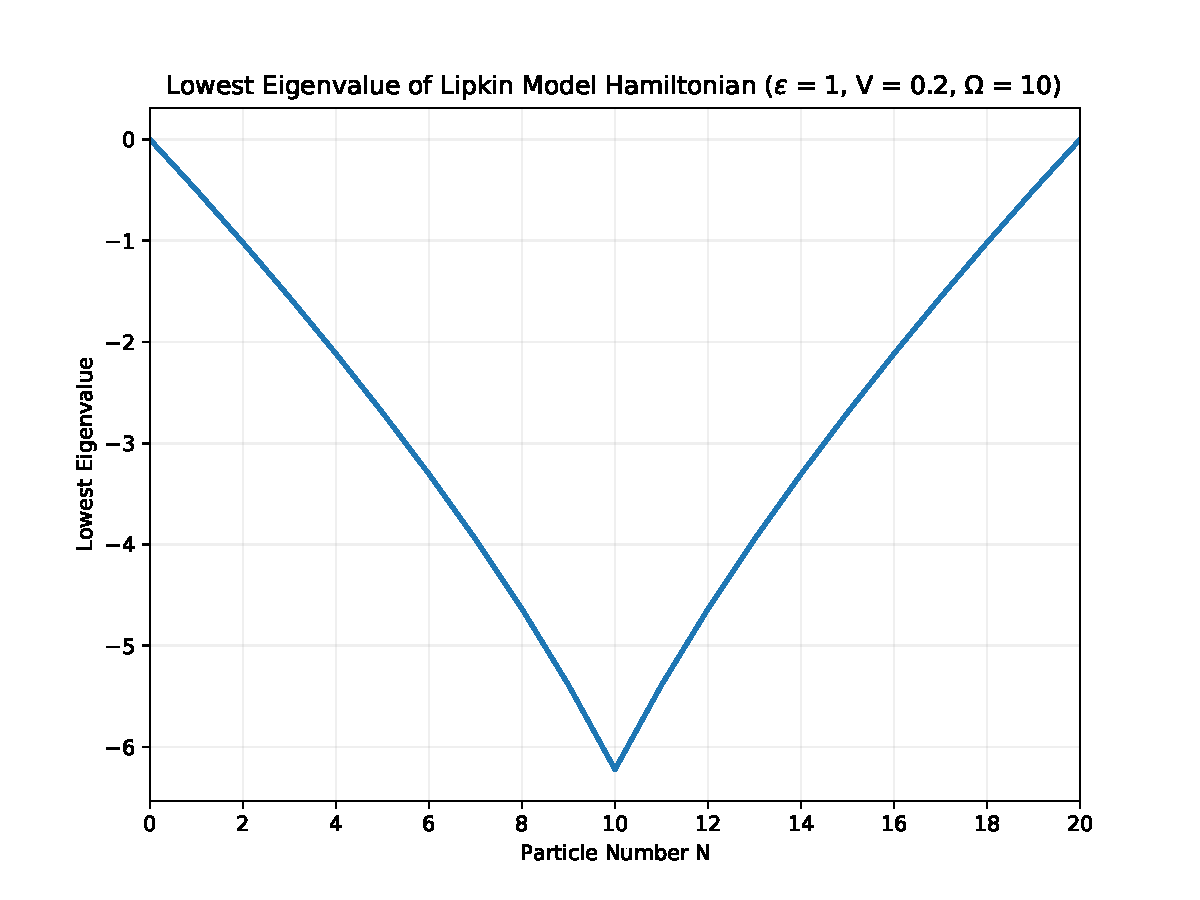
\includegraphics[width=\linewidth]{../figures/plot_lipkin_gs_N.pdf}
  \caption{The ground state energy of the LM hamiltonian for all possible numbers of particles.}
\end{figure}

\begin{figure}
  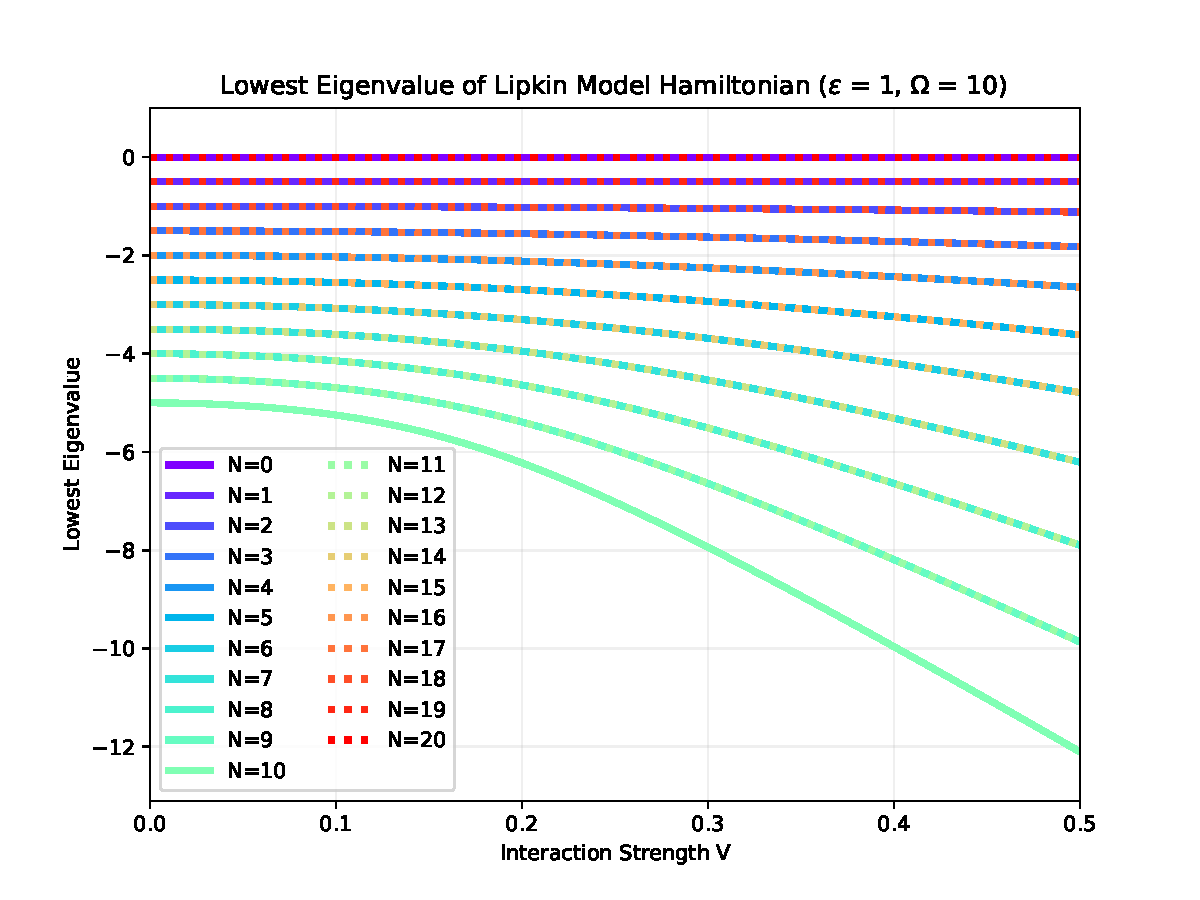
\includegraphics[width=\linewidth]{../figures/plot_lipkin_gs_V_N.pdf}
  \caption{The ground state energy of the LM hamiltonian for various interaction strengths and all numbers of particles.}
\end{figure}

The fundamental symmetries of the Lipkin model lead to symmetries in its spectrum. We can observe one such symmetry in FIG. 2. The lowest energy for $N\leq \Omega$ particles is exactly equal to the lowest energy for $2\Omega-N$ particles, with a minimum at $N=\Omega$. In FIG. 3. we can see that this is a general statement holding true for all values of the interaction parameter $V$. It can be intuitively understood by viewing the holes of the $N$ particle system as the particles of the $2\Omega-N$ system. The full spectrum also exhibits mirror symmetry about zero energy, as depicted in FIG. 4. In other words, each eigenvalue $E > 0$  has a corresponding partner $-E$ with the same values of $K$ and $r$. 

FIG. 4 also demonstrates other interesting properties of the spectrum as the interaction strength changes. For very small values of $V \lesssim 0.05$, the eigenvalues are nearly degenerate and clustered according to signature. Starting from the bottom of the plot, we have 1, 2, ..., 5 lines emerging from the same points at $V=0$. Due to the mirror symmetry in the energies, we then have 5, 4, ..., 1 lines above zero. As V increases, the eigenvalues with the same signature but different $K$ gradually diverge. We encounter the first of many level crossings around $V \approx 0.22$. Eventually the levels will cluster according to $K$ instead of $r$, which can be seen for the lowest (and highest) couple eigenvalues at $V \approx 0.5$. 


\begin{figure*}
  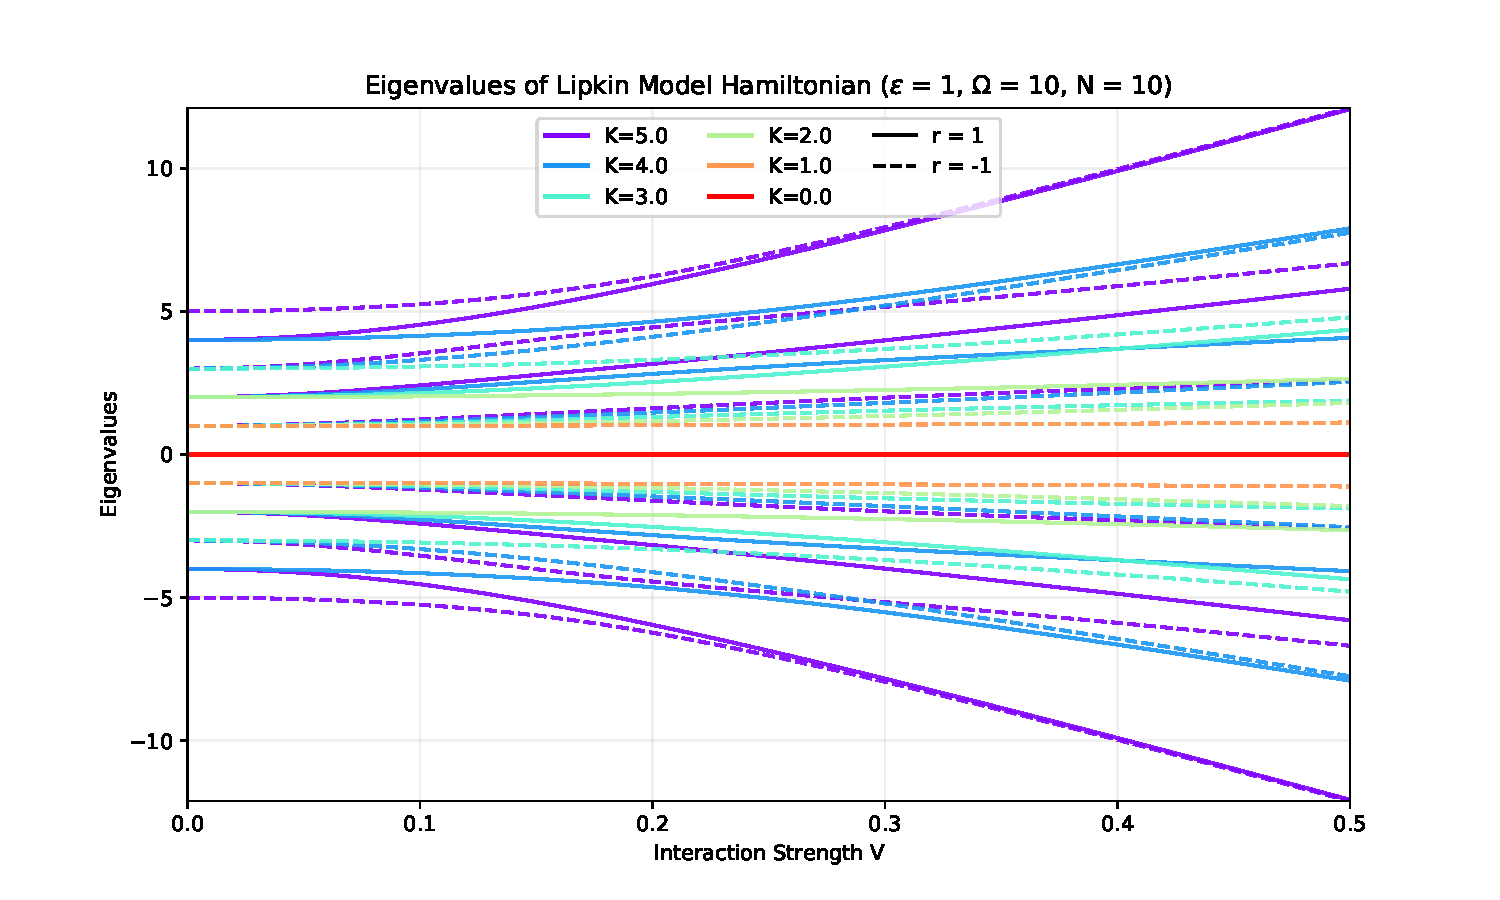
\includegraphics[width=\textwidth]{../figures/plot_lipkin_all_energies.pdf}
  \caption{The eigenvalue spectrum of the LM hamiltonian for various interaction strengths and all numbers of particles.}
\end{figure*}


\subsection{Approximate Methods}

\subsubsection{Hartree-Fock Method}

The first implementations of the nuclear shell model treated nucleons as independent particles moving in an ad-hoc external potential. Simple potentials, such as the harmonic oscillator or the square well, were convenient to work with and provided sufficient justification to further develop the independent-particle picture. The Hartree-Fock (HF) method aims to replace the phenomenologically chosen potential with one derived directly from the two-body interactions. It is based on the variational principle, in which the energy of the system is minimized with respect to the parameters of a physically motivated trial wave function $\ket{\Psi}$:
\begin{equation}
\delta \frac{\bra{\Psi} \hat{H} \ket{\Psi}}{\bra{\Psi}\ket{\Psi}} = 0
\end{equation}
The variational principle guarantees that the minimum energy is an upper bound for the true ground state energy. Thus, it is in our best interest to carefully design a trial wave function that contains as many relevant properties as possible. Whichever design yield a lower energy is automatically a better approximation of the ground state. 

In the Hartree-Fock method, we take the trial wave function to be a Slater determinant with definite particle number $N$. By the Thouless theorem, we can write any particle-number conserving product state as 
\begin{equation}
\ket{\tilde{Z}} = \exp \left( \sum_{ph} \tilde{Z}_{ph}^* a_p^+ a_h \right)  \prod_{i=1}^N a_i^+ \ket{0},
\end{equation}
where the Thouless matrix $\tilde{Z}$ contains the parameters to be tuned. A general two-body hamiltonian in second quantized form is given by 
\begin{equation}
\hat{H} = \sum_{\mu \nu} T_{\mu \nu} a_{\mu}^+ a_{\nu} + \frac{1}{4} \sum_{\mu \lambda \nu \pi} V_{\mu \lambda \nu \pi } a_\mu^+ a_\lambda^+ a_\pi a_\nu.
\end{equation}
Variation of the energy with respect to $\tilde{Z}$ yields the Hartree-Fock equations:
\begin{equation}
[h(\rho_{HF}), \rho_{HF}]=0,
\end{equation}
where the label HF indicates that the relation holds only at the minimum, $\rho=\bra{\tilde{Z}} a_\nu^+ a_\mu \ket{\tilde{Z}}$ is the single-particle density matrix, and $h$ is the single-particle HF hamiltonian defined by
\begin{align}
h(\rho) &\equiv T + \Gamma(\rho), \\
\Gamma_{\mu \nu} &\equiv \sum_{\lambda \pi } V_{\mu \lambda \nu \pi } \rho_{\pi \lambda}.
\end{align}
Here, the single-particle potential $\Gamma$ averages over the two-body interactions and depends on the density matrix. Finally, the Hartree-Fock energy can be written in terms of $\rho$:
\begin{equation}
E_{HF}(\rho) = \frac{1}{2} \Tr (T\rho) + \frac{1}{2} \Tr (h \rho),
\end{equation}
where the minimum occurs when $\rho=\rho_{HF}$. \\


For the half-filled Lipkin model, $N = \Omega$, the calculation simplifies to a 2-dimensional problem due to the $m$-degeneracy:
\begin{equation}
\tilde{Z}_{ph}^* = \tilde{Z}_{m+, m-}^* = \tau \ \ \forall \ \  m=1, ..., \Omega,
\end{equation} 
The complex number $\tau=\tan \frac{\theta}{2} e^{i\phi}$ parameterizes the connection between particle ($\sigma=+1$) and hole ($\sigma=-1$) states. The general product state (16) reduces to an SU(2) coherent state:
\begin{equation}
\ket{\tau} = \frac{1}{(1+|\tau|^2)^{\Omega/2}}e^{\tau \hat{K}_+} \ket{\frac{\Omega}{2}, -\frac{\Omega}{2}}.
\end{equation}
The density matrix can be calculated directly from the anti-commutation relations for the fermion operators $a_\mu^+, a_\mu$:
\begin{equation}
\rho = 
\renewcommand{\arraystretch}{1.2}
\begin{bmatrix}
\cos^2\frac{\theta}{2} & \sin \frac{\theta}{2}  \cos \frac{\theta}{2}  e^{-i\phi}\\
\sin \frac{\theta}{2}  \cos \frac{\theta}{2}  e^{i\phi} & \sin^2\frac{\theta}{2} \\
\end{bmatrix}
,
\end{equation}
From the LM hamiltonian (3) and the density matrix above, we can obtain the self-consistent HF hamiltonian:
\begin{equation}
h = \frac{1}{2} \epsilon \Omega 
\begin{bmatrix}
-1 & \chi \sin \theta e^{i\phi} \\
 \chi \sin \theta e^{-i\phi}& 1
\end{bmatrix}
,
\end{equation}
where we have defined $\chi = \frac{V}{\epsilon}(\Omega-1)$. Then the HF energy (21) is given by
\begin{equation}
E_{HF} (\tau)= -\frac{1}{2} \epsilon \Omega ( \cos \theta + \chi \sin^2 \theta \cos 2\phi ).
\end{equation}

There are (at least) two ways to minimize (26) exactly. The first approach involves imposing the condition for the minimum energy and solving the HF equations (18):
\begin{equation}
-\frac{1}{2} \epsilon \Omega \sin \theta
\begin{bmatrix}
i \chi \sin \theta \sin 2 \phi & e^{-i\phi} - \chi \cos \theta e^{i\phi} \\
\chi \cos \theta e^{-i\phi} - e^{i\phi} & - i \chi \sin \theta \sin 2\phi
\end{bmatrix}
=0.
\end{equation}
The above equation is trivially satisfied for $\theta_{HF} = 0$. In this case, the choice of $\phi_{HF}$ is irrelevant since $\tau_{HF}=0$ anyway, so we will just set $\phi_{HF}$ to zero as well. For $\theta_{HF} \neq 0$, the diagonal elements imply that we must have $\phi_{HF}=0$. Then the off-diagonal elements give $1=\chi \cos \theta_{HF}$, which only has solutions for $\chi \geq 1$. Therefore, the HF solution is
\begin{align}
\begin{split}
\phi_{HF} = 0, \ \ \
\theta_{HF} = \begin{cases} 
      0, & \chi < 1,\\
      \cos^{-1} \chi^{-1}, & \chi \geq 1.
   \end{cases}
\end{split}
\end{align}
and the minimum energy is
\begin{align}
\begin{split}
E_{HF} = \begin{cases} 
      -\frac{1}{2}\epsilon \Omega & \chi < 1,\\
       -\frac{1}{4}\epsilon \Omega (\chi + \chi^{-1}) & \chi \geq 1.
   \end{cases}
\end{split}
\end{align}

\begin{figure}
  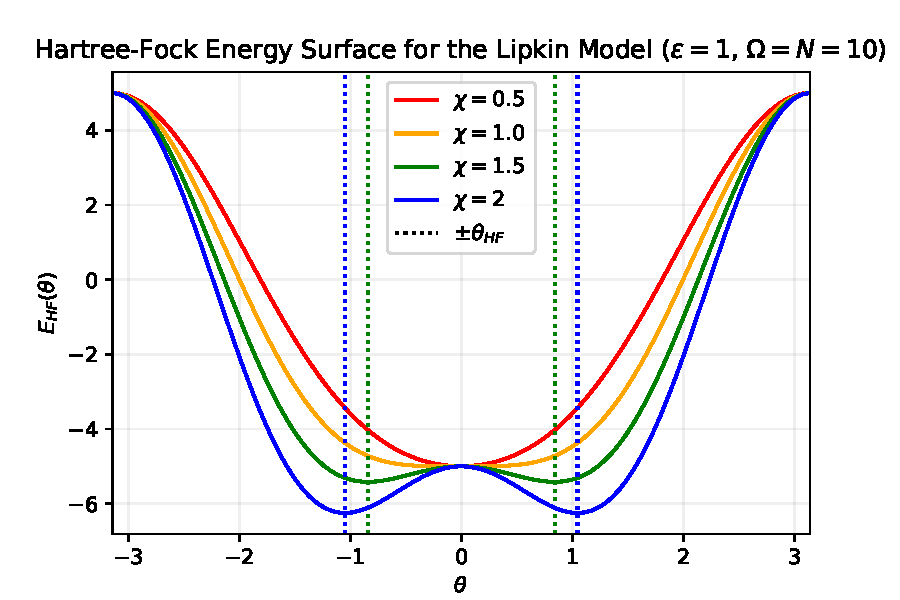
\includegraphics[width=\linewidth]{../figures/plot_hf_surface.pdf}
  \caption{Hartree-Fock energy surface for the Lipkin model with various values of $\chi$.}
\end{figure}

This HF solution points to a few drawbacks of the Hartree-Fock method. First, the averaging of the two-body interaction only improves the calculation of the LM ground state energy beyond a critical value of $\chi_c = 1$.  Next, the condition $1=\chi \cos \theta_{HF}$ for $\chi > \chi_c$ actually implies that there are two degenerate solutions at $\theta_{HF}$ and $-\theta_{HF}$, separated by a barrier which increases in height as $\chi$ increases. FIG. 5 shows these two solutions along with the HF energy surface for values of $\chi$ below and above $\chi_c$. 


\begin{figure*}
  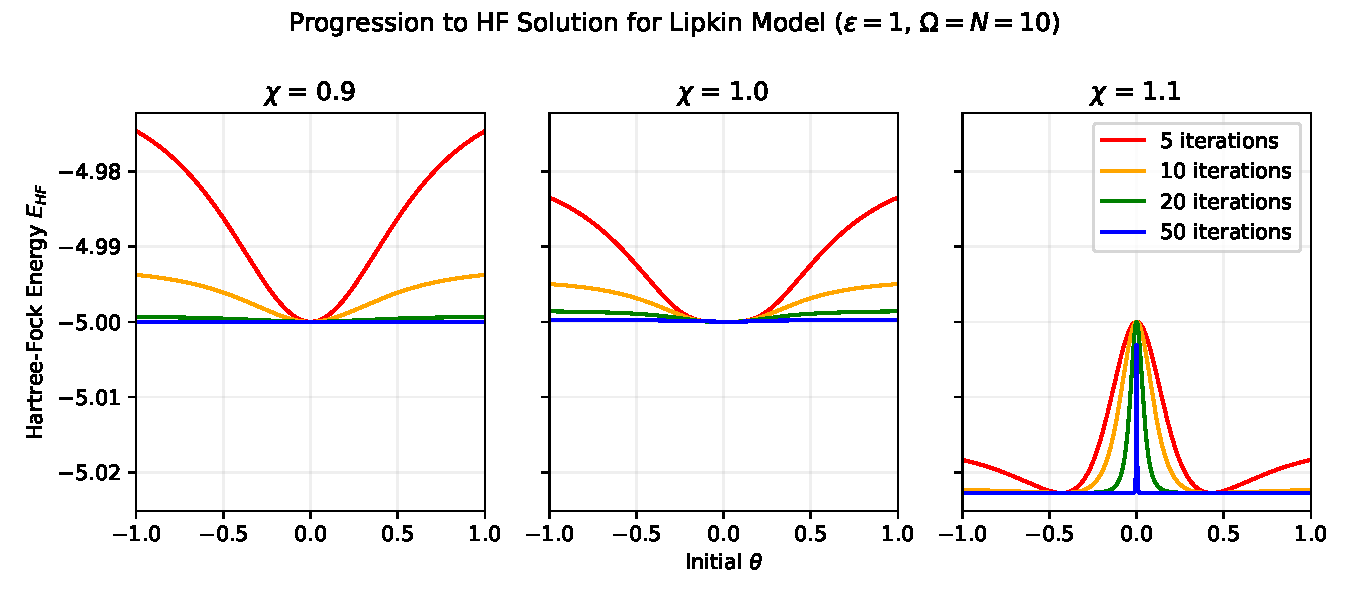
\includegraphics[width=\textwidth]{../figures/plot_hf_iter.pdf}
  \caption{INSERT A CAPTION HERE}
\end{figure*}

When we solve the $\chi>\chi_c$ problem numerically, we will necessarily have to choose one of the two minima, not both. The solution we choose depends on the initial choice of $\theta$ and will become the ground state, while the other will become the first excited state due to tunneling effects through the finite barrier. This signals a broken symmetry in the HF solution for the Lipkin model.

In practice, the Hartree-Fock equations (18) are solved iteratively. Starting with some initial value of $\theta$, one constructs and diagonalizes the self-consistent HF hamiltonian $h$ (25):
\begin{equation}
h \ket{v^{(\lambda)}} = \epsilon_{\lambda} \ket{v^{(\lambda)}} , \ \ \lambda = h, p. 
\end{equation}
Then, the eigenvector of $h$ corresponding to the hole state is used to calculate the density matrix $\rho$ via
\begin{equation}
\rho = \ket{v^{(h)}} \bra{v^{(h)}},
\end{equation}
and the result is used to calculate the single particle potential $\Gamma$ and update the HF hamiltonian $h$. This process is repeated until self-consistency is achieved. Note that this method only requires the explicit form of $h$ (25) in the first iteration. The following iterations simply solve the eigenvalue problem to construct a new hamiltonian. 

The dependence on the initial value of $\theta$ in the early stages of this iterative scheme is shown in FIG. 6 for $\chi$ below, at, and above $\chi_c$. For $\chi \leq \chi_c$, convergence around the HF minimum $\theta_{HF} = 0$ is rapid. This behavior is supported by the shape of the HF energy surface in FIG. 5. For $\chi > \chi_c$, however, the saddle point at $\theta=0$ causes convergence issues. Thus, choosing an initial value of $\theta$ sufficiently away from saddle points is recommended. 

Another way to minimize (26) exactly involves explicitly calculating the gradient of $E_{HF}$ with respect to $\tau$ and requiring that it vanishes. The gradient is given by
\begin{align}
\frac{\partial E_{HF}}{\partial \theta } &= \frac{1}{2} \epsilon \Omega \sin \theta (1-\chi \cos\theta \cos 2\phi),\\
\frac{\partial E_{HF}}{\partial \phi } &= \frac{1}{2} \epsilon \Omega \sin \theta \sin 2\phi,
\end{align}
and setting both equations equal to zero returns the same solutions as before. The numerical counterpart to this approach is to minimize $E_{HF}$ using gradient descent. 


\subsubsection{Signature Projection}

In the previous section, we briefly mentioned signs of spontaneous symmetry breaking in the HF solution for the Lipkin model. We will now identify the broken symmetry: signature. To calculate the signature of a deformed Hartree-Fock state (24), it is convenient to use the generating function:
\begin{align}
\begin{split}
\bra{\tau} e^{\alpha_- \hat{K}_-} & e^{\alpha_0 \hat{K}_0}  e^{\alpha_+ \hat{K}_+}
\ket{\tau'} \\
=&\frac{1}{(1+|\tau|^2)^{\Omega/2}} \frac{1}{(1+|\tau'|^2)^{\Omega/2}}\\
&\left( e^{-\frac{1}{2}\alpha_0} + e^{\frac{1}{2}\alpha_0} (\tau^* + \alpha_{-}) (\tau' +\alpha_+) \right)^\Omega
\end{split}.
\end{align}
Then the expectation value of the signature operator (14) is straightforward to obtain:
\begin{align}
\begin{split}
\bra{\tau} \hat{R} \ket{\tau} = e^{-i \pi \Omega/2} \cos^\Omega \theta=
r_{g.s.}
\begin{cases} 
      1 & \chi < 1,\\
       \chi^{-\Omega}& \chi \geq 1.
   \end{cases}
\end{split}.
\end{align}
As $\chi$ increases beyond $\chi_c$, the signature decays from the ground state value to zero. Since we know the exact LM states have good signature, we can attempt to restore the signature symmetry in the HF solution by introducing the signature projection operator
\begin{align}
\hat{P}_r = \frac{1}{2} (1+r\hat{R}),\\
\ket{\Psi_r} \equiv \hat{P}_r \ket{\Psi}, \\
 \hat{R}\ket{\Psi_r} = r \ket{\Psi_r}.
\end{align}
The expectation value of the hamiltonian in the extracted state with good signature is called the signature-projected energy:
\begin{equation}
E_r = \frac{\bra{\Psi_r} \hat{H} \ket{\Psi_r}}{\bra{\Psi_r} \ket{\Psi_r}}.
\end{equation}
For the LM hamiltonian, the generating function yields 
\begin{align}
E_r(\tau) &= E_{HF}(\tau) W_r(\tau),
\end{align}
where the $r$-dependence is contained in a numerical factor we will refer to as the signature weight
\begin{equation}
W_r(\tau) = \frac{1+r r_{g.s.} \cos^{\Omega-2} \theta}{1+r r_{g.s.} \cos^\Omega \theta}.
\end{equation}




Since the projected energy can be calculated by scaling the HF energy by the signature weight, it is simple to obtain modest improvements for the ground state energy ($r=r_{g.s.}$) and the 1st excited state energy ($r=-r_{g.s.}$). This projection-after-variation (PAV) method lowers the ground state energy around $\chi \approx 1-2$, but is restricted by the HF solution it builds on. For instance, PAV cannot lower the HF energy for $\chi < \chi_c$ because the signature weight is 1 for $\theta_{HF}=0$. PAV is also characterized by sharp kinks at $\chi_c$, due to the sudden jumps in the signature weight for the HF solution (see FIG. 7).

\begin{figure}
  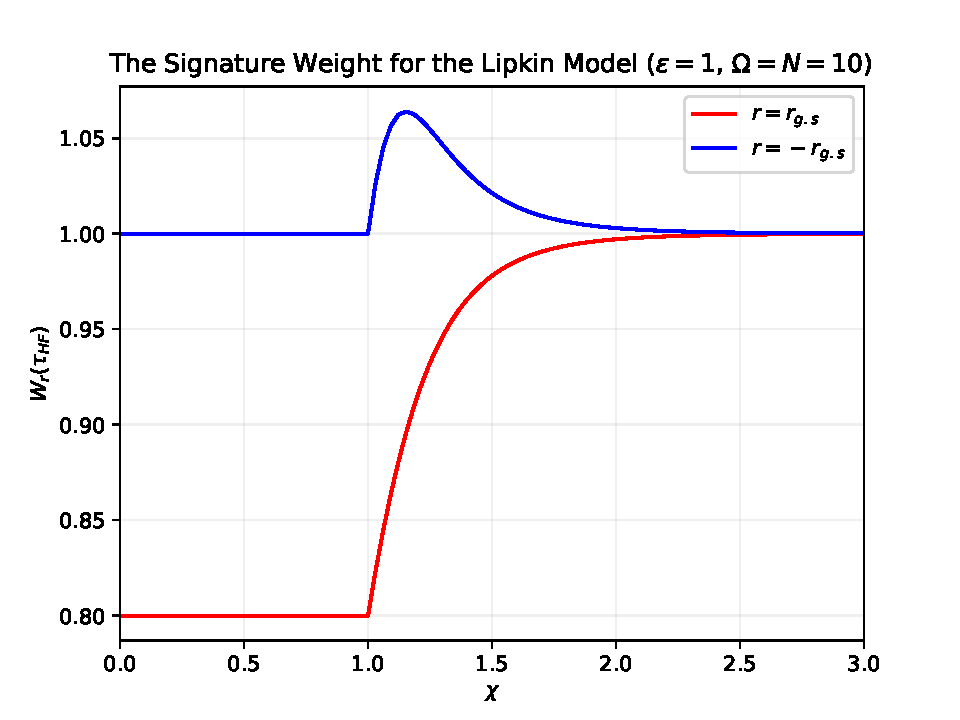
\includegraphics[width=\linewidth]{../figures/plot_weight.pdf}
  \caption{CAPTION.}
\end{figure}

The broken signature symmetry is better handled by variation-after-projection (VAP), i.e. minimizing $E_r(\tau)$ directly. In addition to the derivatives of $E_{HF}(\tau)$ in equations (33) and (34), we will need the derivative of the signature weight:
\begin{equation}
\frac{\partial W_r}{\partial \theta} = \frac{r r_{g.s.} \cos^{\Omega-3} \theta \sin \theta}{(1+r r_{g.s.} \cos^\Omega \theta)^2}
 \left( 2(1+r r_{g.s.} \cos^\Omega \theta)-\Omega \sin^2\theta \right),
\end{equation}
Then the gradient of $E_r(\tau)$ is given by
\begin{align}
\frac{\partial E_r}{\partial \theta}&= E_{HF}(\tau) \frac{\partial W_r}{\partial \theta} + \frac{\partial E_{HF}}{\partial \theta} W_r(\tau),\\
\frac{\partial E_r}{\partial \phi}&=  \frac{\partial E_{HF}}{\partial \phi} W_r(\tau),
\end{align}
and we may then proceed with the usual gradient descent. For $r=-r_{g.s.}$ and small $\theta$, the calculation of the signature weight and its derivative can become unstable. To mitigate floating point errors, we can use the Taylor expansions in place of the direct formulas when needed:
\begin{align}
W_{-r_{g.s.}} &\approx \frac{\Omega-2}{\Omega},\\
\frac{\partial W_{-r_{g.s.}}}{\partial \theta}& \approx \frac{\Omega-2}{\Omega} \theta.
\end{align}
The PAV and VAP energies are compared to the HF energy in FIG??????
talk about how much better the vap energies are



\subsubsection{Generator Coordinate Method}

The generator coordinate method (GCM) is yet another variational approach to the many-body problem. The trial wave function is a continuous superposition of Hartree-Fock-Bogoliubov states, the most general ansatz among those discussed in this review. We will formulate GCM in terms of the Lipkin model and take the generating functions to be the particle number-conserving product states we have employed thus far:
\begin{equation}
\ket{\Psi} = \int d\theta f(\theta) \ket{\theta}.
\end{equation}
Here we have taken $\tau$ to be real,  $\ket{\tau} = \ket{\theta}$, which will be sufficient for our application. In principle, this horizontal expansion can be extended to any number of generator coordinates. 

The weight function $f(\theta)$ acts as the expansion coefficients for the ansatz. Variation with respect to $f(\theta)$ produces the Hill-Wheeler (HW) equation:
\begin{equation}
\int d\theta' H(\theta, \theta') f(\theta') = \int d \theta' N(\theta, \theta') f(\theta'),
\end{equation}
where 
\begin{align}
H(\theta, \theta') &= \bra{\theta} \hat{H} \ket{\theta}, \\
N(\theta, \theta') &= \bra{\theta}\ket{\theta},
\end{align}
are the hamiltonian and norm kernels, respectively. The HW equation constitutes a generalized eigenvalue problem,
\begin{equation}
Hf = ENf,
\end{equation}
which normally cannot be solved by inverting the norm kernel since it is often singular. Luckily, this is not the case for the Lipkin model:
\begin{align}
\begin{split}
N(\theta, \theta') &= \cos^\Omega \left( \frac{\theta-\theta'}{2} \right)\\
&= \frac{1}{2^\Omega} \left( e^{\frac{1}{2}i(\theta-\theta')} + e^{-\frac{1}{2}i(\theta-\theta')}  \right)^\Omega\\
&= \frac{1}{2^\Omega}  \sum_{k = 0}^\Omega {\Omega\choose k} \left( e^{\frac{1}{2}i(\theta-\theta')} \right)^k \left( e^{-\frac{1}{2}i(\theta-\theta')} \right)^{\Omega-k}\\
&= \frac{1}{2^\Omega}  \sum_{k = -\Omega/2}^{\Omega/2} {\Omega\choose k+\Omega/2} \left( e^{\frac{1}{2}i(\theta-\theta')} \right)^{k} \left( e^{-\frac{1}{2}i(\theta-\theta')} \right)^{-k} \\
&= \frac{2\pi}{2^\Omega}  \sum_{k = -\Omega/2}^{\Omega/2} {\Omega\choose k+\Omega/2} \frac{e^{ik\theta}}{\sqrt{2\pi}} \frac{e^{-ik\theta'}}{\sqrt{2\pi}}
\end{split}
\end{align}
In fact, the above shows that the eigenvalues $n_k$ of the norm kernel are not only strictly positive
\begin{equation}
n_k = \frac{2\pi}{2^\Omega} {\Omega\choose k+\Omega/2} > 0,
\end{equation}
but the associated $\Omega+1$ functions
\begin{equation}
u_k(\theta) = \frac{e^{-ik\theta}}{\sqrt{2\pi}},
\end{equation}
form a complete, orthonormal basis in which $N$ can be expanded. Since $N$ is positive definite, it also has a well-defined decomposition $N=N^{1/2} N^{1/2}$ which can be expanded in the same basis
\begin{equation}
N^{1/2}(\theta, \theta')= \sum_{k = -\Omega/2}^{\Omega/2} \sqrt{n_k} u_k(\theta) u_k^* (\theta').
\end{equation}
Then the generalized eigenvalue problem can be written as
\begin{equation}
N^{1/2} H N^{1/2} g = E g,
\end{equation}
with $f = N^{-1/2}g$.

The functions $u_k(\theta)$ motivate the introduction of "natural states"
\begin{equation}
\ket{k} = \frac{1}{\sqrt{n_k}} \int d\theta u_k(\theta) \ket{\theta},
\end{equation}
which span the collective subspace of Hilbert space containing the generating states $\ket{\theta}$. Projecting onto this subspace transforms (57) into a discrete eigenvalue problem of dimension $\Omega+1$:
\begin{align}
&\sum_{k'}\hat{H}_{k,k'} g_{k'} = E g_k,\\
\hat{H}_{k,k'} = &\frac{1}{2\pi} \int d\theta d\theta' \frac{e^{ik\theta}}{\sqrt{n_k}} H(\theta, \theta) \frac{e^{-ik'\theta'}}{\sqrt{n_{k'}}}\\
\begin{split}
H(\theta, \theta') = &-\frac{1}{2}\epsilon \Omega N(\theta, \theta') \left[ \frac{\cos\left( \frac{\theta+\theta'}{2} \right)}{\cos\left( \frac{\theta-\theta'}{2} \right)} \right.\\
&+\left.
\frac{\chi}{2} \left( \frac{1+\sin^2\left( \frac{\theta+\theta'}{2} \right)}{\cos^2\left( \frac{\theta-\theta'}{2} \right)}-1 \right)
\right]
\end{split}
\end{align}

The GCM wave function is then given by
\begin{equation}
\ket{\Psi} = \sum_k g_k \ket{k},
\end{equation}
the collective wave functions by
\begin{equation}
g(\theta) = \sum_k g_k u_k(\theta),
\end{equation}
and the weight functions by
\begin{equation}
f(\theta) = \sum_k \frac{g_k}{\sqrt{n_k}} u_k(\theta).
\end{equation}

\begin{figure*}
  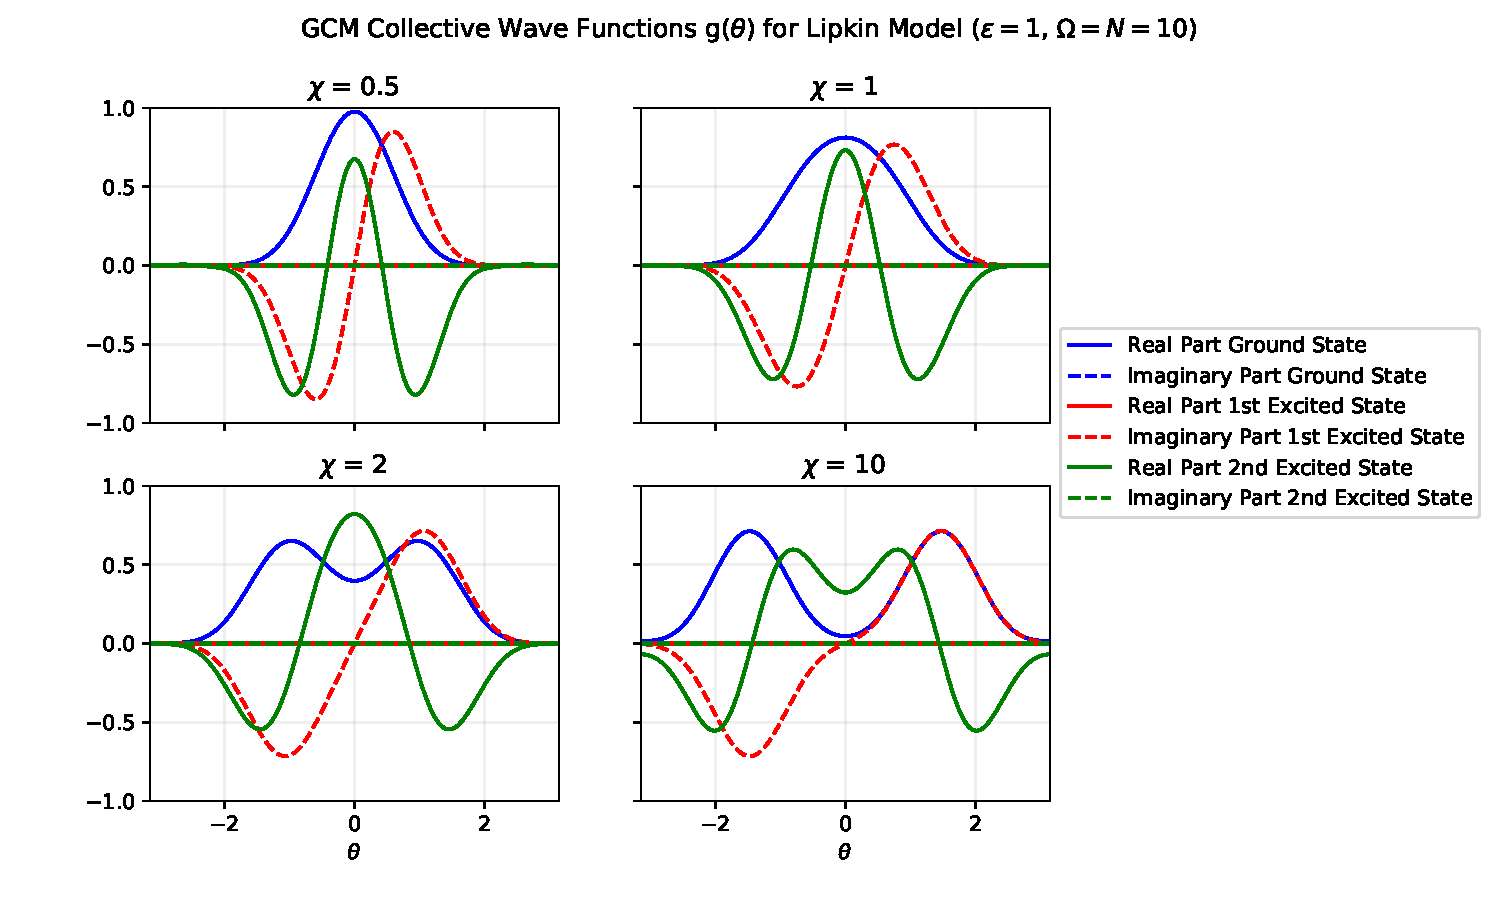
\includegraphics[width=\textwidth]{../figures/plot_gcm_wvfuncs.pdf}
  \caption{INSERT A CAPTION HERE}
\end{figure*}

The lowest three collective wave functions are plotted in FIG. 8 for various values of $\chi$. The ground state and the 2nd excited state are both real and even in $\theta$, while the 1st excited state is imaginary and odd. For $\chi \leq \chi_c$, the ground state is a Gaussian distribution about the Hartree-Fock minimum $\theta_{HF} = 0$. The HF solution clearly contributes the most to the GCM ground state, but the width of the distribution is rather large, suggesting the HF solution is a significant simplification of the full picture. As $\chi$ passes the critical threshold, the GCM wave functions spread out and develop twin peaks. For the ground state, these peaks correspond to the two HF minima at $\pm \theta_{HF}$. Since contributions from both minima (and the surrounding regions) are considered, the GCM states do not break signature symmetry like the HF states. All of the ground states in FIG. 8 involve some contribution from the $\theta=0$ product, even when $\chi$ is very large. For $\chi = 10$, another interesting feature appears. The GCM ground state and first excited state overlap almost perfectly for $\theta>0$ and are mirror images of one another for $\theta<0$. This is reminiscent of how the states with the same $K$ but opposite signature become degenerate for large interaction strengths in FIG. 4.

\subsubsection{Summary}

In FIG. 9, the two lowest energies from each of the methods applied to the Lipkin model are plotted together. The Hartree-Fock method produces a ground state energy that roughly captures the qualitative behavior of the exact ground state. Projecting good signature onto the HF solution provides the PAV estimations for the ground state and excited state energies. The PAV curves are the only ones with kinks, but this is to be expected since the signature weight for the HF solution varies rapidly around $\chi_c$. The PAV and VAP energies demonstrate the clustering of the two lowest states with opposite signature, but 

for $\chi>2$, there is little improvement compared to the HF energy. GCM is by far the most effective method of the bunch. Its predictions are nearly indistinguishable from the exact solutions. 

\begin{figure*}
  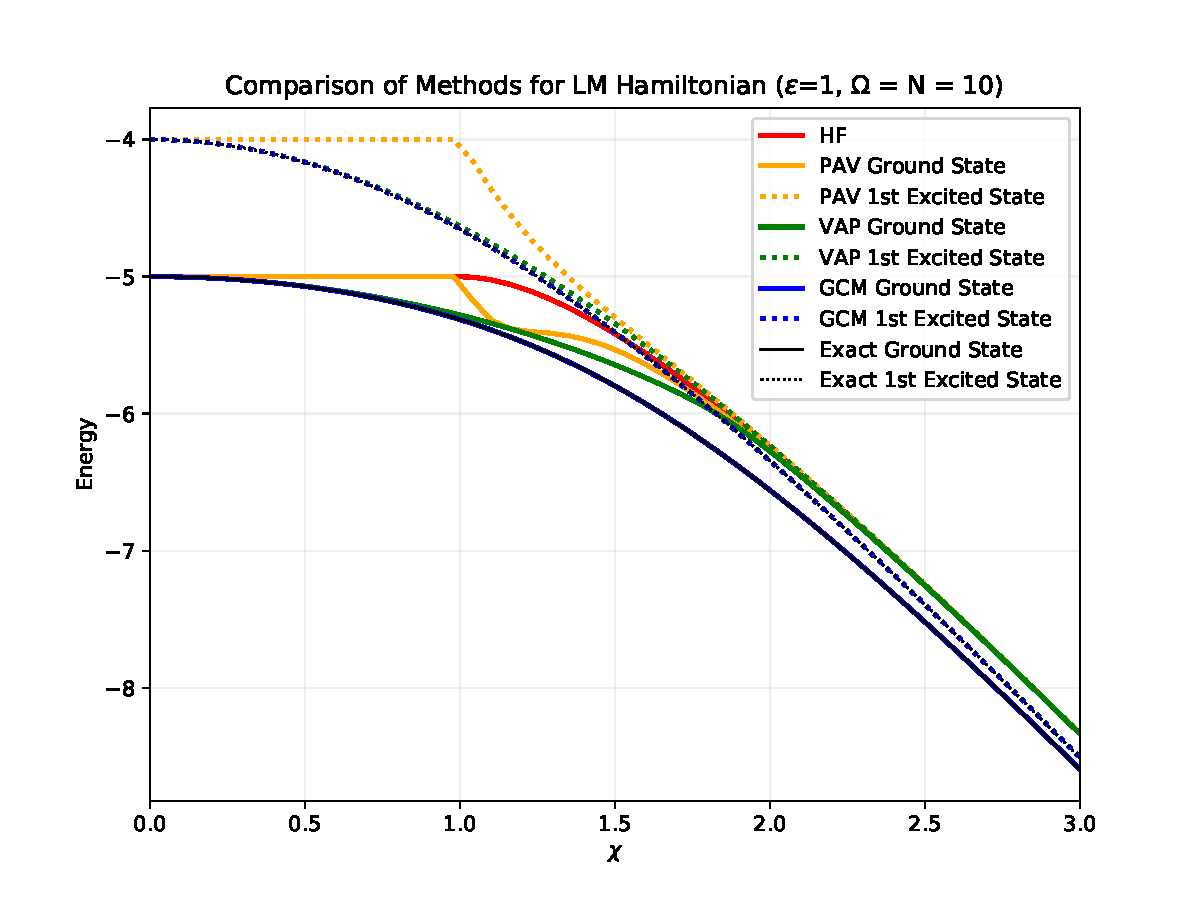
\includegraphics[width=\textwidth]{../figures/plot_lipkin_energies.pdf}
  \caption{INSERT A CAPTION HERE}
\end{figure*}

\section{SENIORITY MODEL}

In the previous section, the Hartree-Fock method partially handled the particle-hole correlations due to the long-range component of the nucleon-nucleon interaction. On the other hand, the short-range component results in particle-particle correlations which cannot be accounted for by pure Hartree-Fock. These pairing correlations are important to consider, since they help us understand many additional nuclear properties, such as the odd-even effect and the existence of an energy gap in the low-lying nuclear spectra.

The short-range interaction is most active between nucleons with equal $|m|$ but opposite sign, because the spatial overlap is maximal. This motivates the form of the seniority model hamiltonian:
\begin{equation}
H = -G \sum_{m,m'>0} a_{m'}^+ a_{-m'}^+ a_{-m} a_m,
= -GS_+ S_-,
\end{equation}
with 
\begin{align}
S_+ = \sum_{m>0} a_m^+ a_{-m}^+, \\
S_- = (S_+)^+,
\end{align}
where we imagine placing $N$ nucleons in a single $j$-shell at zero energy.

\subsection{Exact Method}
\subsubsection{Quasi-Spin}

Similar to how we solved the Lipkin model, we introduce pairing quasi-spin operators
\begin{align}
\hat{s}_+^{(m)} &= a_m^+ a_{-m}^+,\\
\hat{s}_-^{(m)} &=  a_{-m} a_m,\\
\hat{s}_0^{(m)} &= \frac{1}{2} (a_m^+ a_m + a_{-m}^+ a_{-m} -1),
\end{align}
that satisfy the commutation relations of angular momenta
\begin{align}
[s_+^{(m)}, s_-^{m}] &= 2s_0^{(m)}, \\
[s_0^{(m)}, s_+^{m}] &= s_+^{(m)}, \\
[s_0^{(m)}, s_-^{m}] &= -s_-^{(m)}. 
\end{align}
The seniority hamiltonian can then be written as
\begin{equation}
H = -G(\hat{\vec{S}} \cdot \hat{\vec{S}} - \hat{S}^2_0 + \hat{S}_0),
\end{equation}
where 
\begin{equation}
\hat{\vec{S}} = \sum_{m>0} \hat{\vec{s}}^{(m)}
\end{equation}
is the total quasi-spin operator and
\begin{equation}
S_0 = \frac{1}{2} (\hat{N}-\Omega)
\end{equation}
is its z-component. Then the total energy of the system can be written in terms of the total quasi-spin S:
\begin{equation}
E(S) = -G \left( S(S+1) -\frac{1}{4}(N-\Omega)^2 + \frac{1}{2}(N-\Omega) \right).
\end{equation}


Let us define the seniority quantum number $s$ by 
\begin{equation}
S = \frac{1}{2} (\Omega-s),
\end{equation}
where 
\begin{align}
\begin{split}
 s = \begin{cases} 
      0, 2, 4, ..., N & \text{for N even},\\
      1,3,5, ... N & \text{for N odd},
   \end{cases}
\end{split}
\end{align}
Translating (77) using relation (78) gives the total energy as a function of seniority:
\begin{equation}
E(N,s) = -\frac{G}{4} (s^2-2s(\Omega+1)+2N(\Omega+1) - N^2)
\end{equation}



\subsection{Approximate Method}
\subsubsection{Bardeen-Cooper-Schrieffer}


\begin{figure}
  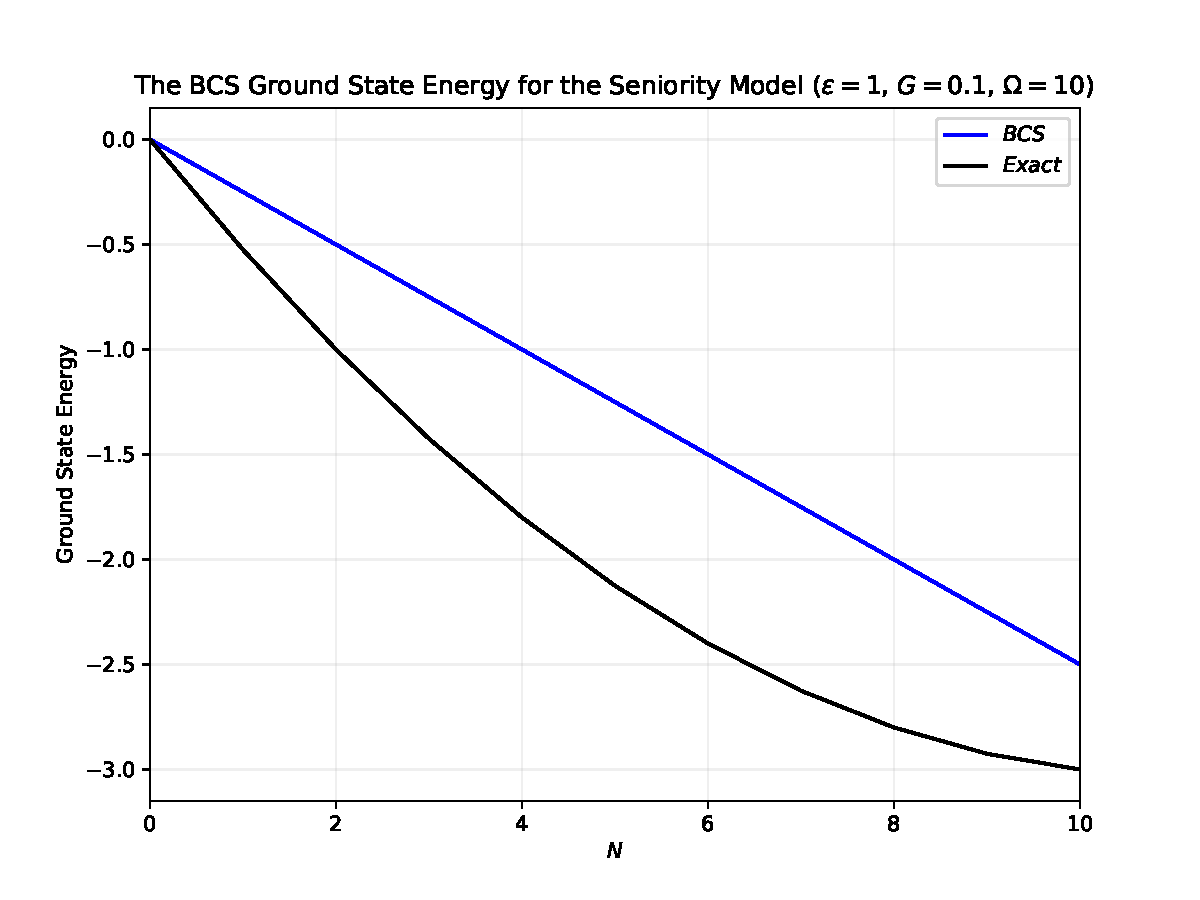
\includegraphics[width=\linewidth]{../figures/plot_bcs_energy.pdf}
  \caption{cap}
\end{figure}

\begin{figure}
  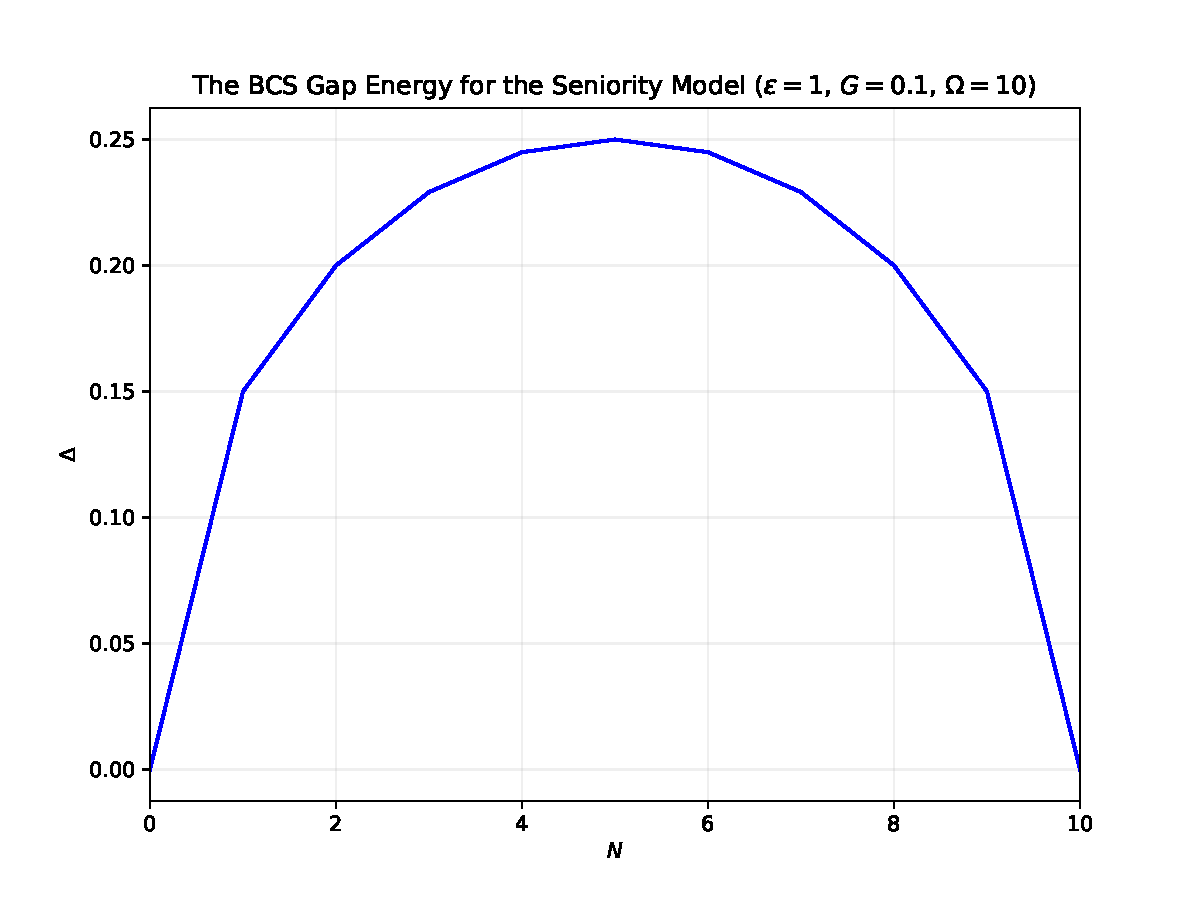
\includegraphics[width=\linewidth]{../figures/plot_bcs_gap.pdf}
  \caption{cap}
\end{figure}
\section{Conclusion}

power of variational principle- guarantee
most useful when trial wave function bakes in symmetries of the problem

\begin{thebibliography}{9}
\bibitem{latexcompanion} 
Michel Goossens, Frank Mittelbach, and Alexander Samarin. 
\textit{The \LaTeX\ Companion}. 
Addison-Wesley, Reading, Massachusetts, 1993.

\bibitem{einstein} 
Albert Einstein. 
\textit{Zur Elektrodynamik bewegter K{\"o}rper}. (German) 
[\textit{On the electrodynamics of moving bodies}]. 
Annalen der Physik, 322(10):891–921, 1905.

\bibitem{knuthwebsite} 
Knuth: Computers and Typesetting,
\\\texttt{http://www-cs-faculty.stanford.edu/\~{}uno/abcde.html}
\end{thebibliography}


\end{document}